\documentclass[conference]{IEEEtran}
\IEEEoverridecommandlockouts

\usepackage{cite}
\usepackage{amsmath,amssymb,amsfonts}
\usepackage{graphicx}
\usepackage{textcomp}
\usepackage{xcolor}
\usepackage{url}
\usepackage[hidelinks]{hyperref}

\begin{document}

\title{A Computational Comparison of Prototype, Exemplar, and\\
Rule-Based Models of Human Category Learning}

\author{\IEEEauthorblockN{Rabea Abdelwahab}
\IEEEauthorblockA{\textit{CS 6795: Cognitive Science} \\
\textit{Georgia Institute of Technology}\\
Summer 2026}}

\maketitle

\begin{abstract}
I implement three computational models of concept representation---a prototype
model, an exemplar model, and a rule-based model---and evaluate which of them
reproduces the human difficulty ordering of the six Shepard, Hovland, and
Jenkins (SHJ) category structures. The criterion is behavioral rather than
accuracy-based; a model succeeds to the extent that the structures difficult
for it are the structures difficult for people, reproducing the ordering
$\text{I} < \text{II} < \{\text{III},\text{IV},\text{V}\} < \text{VI}$ and, in
particular, the comparatively early mastery of the two-dimensional Type~II
structure. Each model is implemented as an online learner and trained under the
errors-to-criterion paradigm, and the exemplar model is realized as ALCOVE so
that its selective attention is learned trial by trial rather than fixed in
advance. I find that only the exemplar model with learned attention reproduces
the ordering, including the Type~II advantage; freezing attention removes that
advantage while leaving the remainder of the ordering intact, which localizes
the Type~II effect to dimensional attention rather than to exemplar storage as
such. The prototype model cannot separate Types~II and~VI, whose category means
coincide, and the rule model masters Type~I almost immediately yet finds Type~II
hard, inverting the human pattern. These results support an
exemplar-plus-attention account of human category learning.
\end{abstract}

\begin{IEEEkeywords}
category learning, concept representation, exemplar models, selective attention,
Shepard--Hovland--Jenkins, cognitive modeling
\end{IEEEkeywords}

\section{Introduction}
\label{sec:intro-ref}
Concept learning is a problem of representation before it is a problem of
statistics. A learner who has seen a few members of a category can classify the
next member without a definition, and contemporary machine systems approach that
competence only in part \cite{lake2015}. Recent comparisons of language-model
embeddings against human categorization data find that machine representations
align with human category boundaries at a coarse level and diverge on the finer
structure of a concept \cite{vemuri2025}. The question of which representational
format best matches human generalization is therefore current rather than
historical; it constrains what a more human-aligned representation would have to
be.

This project concerns mental representation, which is the central commitment of
the computational and representational understanding of mind that frames the
course \cite{thagard2005,goel2026}. Cognitive science offers three durable accounts of
what is stored when a person holds a concept, and each is a claim about the mind
rather than a choice of algorithm. The prototype account holds that a category
is summarized by an abstracted central tendency that need never have been
observed \cite{rosch1975,posner1968}. The exemplar account holds that no summary
is stored, and that classification is a judgment of similarity to remembered
instances \cite{medin1978,nosofsky1986}. The rule account holds that a concept
is an explicit condition on features, acquired by hypothesis testing
\cite{bruner1956}. Because the three accounts predict different patterns of
generalization, they can be separated by evidence rather than left to agree.

I state the research question so that it can fail: among prototype, exemplar, and
rule representations, which one best reproduces the way people generalize
categories learned from a handful of examples, measured against the human
difficulty ordering of the six SHJ category structures \cite{shepard1961}?
People learn the six structures in a stable order of difficulty, and that
order---recovered under controlled replication \cite{nosofsky1994}---is the
behavioral signature that any account of human concepts must reproduce. I treat
reproducing the ordering as necessary and treat raw classification accuracy as
helpful but not sufficient; a model that classifies accurately while misordering
the structures has failed the cognitive claim. The Type~II structure is the
sharpest part of the test, because people master it earlier than its number of
relevant dimensions would predict, and a model that cannot recover that anomaly
cannot be said to generalize as people do.

\section{Model/Tool Design}
The tool is a small Python codebase with three parts: an encoding of the SHJ
stimuli, the three models, and a runner that trains and scores each under matched
conditions. I used NumPy for the numerical work and Matplotlib for the figures,
and the analysis is packaged as a reproducible notebook so that every reported
number and figure is regenerated from a single fixed random seed. The design is
driven by theory rather than by engineering convenience; the differences among
the models are intended to be the differences among the accounts of
Section~\ref{sec:intro-ref}, and each model shares a common training interface so
that the runner treats them identically.

The stimuli are the eight objects that vary on three binary dimensions,
partitioned into two categories of four. Up to relabeling of the dimensions and
the categories there are exactly six such partitions, and I do not take that fact
on trust; the test suite enumerates every four-against-four split of the stimulus
set, groups the splits into symmetry classes, and confirms that the six encoded
types match the SHJ structural invariants of relevant dimensions, linear
separability, and cohesion (Fig.~\ref{fig:struct}). Encoding the structures by
verification rather than by transcription removes a class of silent error that
would otherwise be indistinguishable from a modeling result.

\begin{figure}[t]
\centering
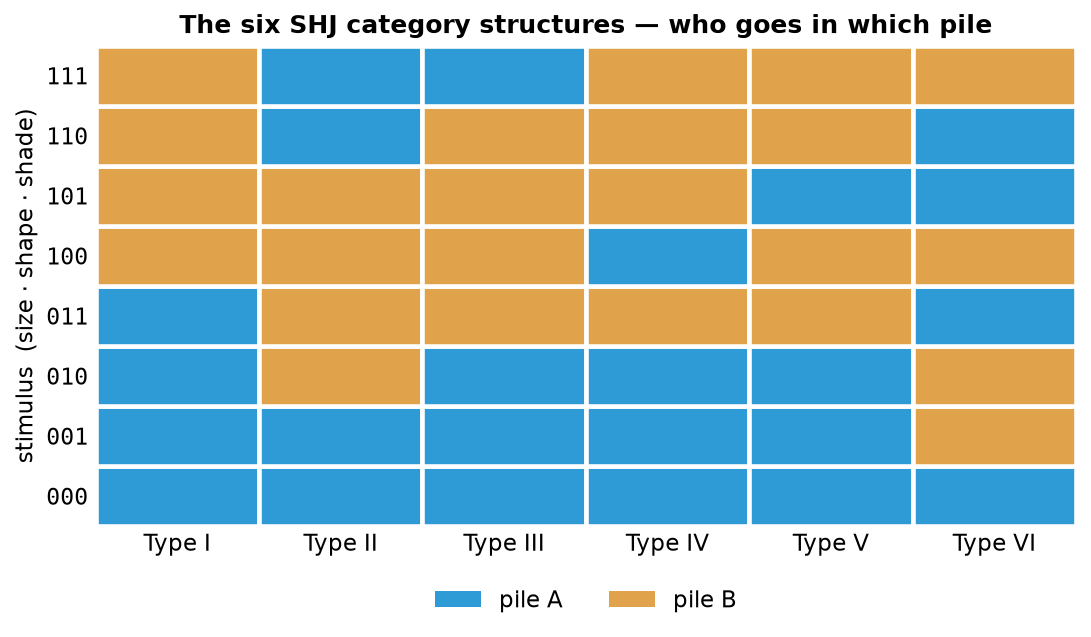
\includegraphics[width=\columnwidth]{../figures/fig0_structures.png}
\caption{The six SHJ category structures. Rows are the eight stimuli, given as
three-bit codes; columns are the six types; cell color is the assigned category.
The partitions are verified by exhaustive enumeration rather than transcribed.}
\label{fig:struct}
\end{figure}

The prototype model stores one summary point per category and classifies by
similarity to it \cite{rosch1975,posner1968}. Each category's prototype is the
running mean of the instances assigned to it, and the probability of a category
is a Luce choice over the similarities of the probe to the two prototypes. This
model predicts a specific failure: when the two category means coincide, as they
do for the XOR-like Type~II and the parity-based Type~VI, the prototypes are
indistinguishable and the model remains at chance regardless of training.

The exemplar model stores every training instance and classifies a probe by its
summed, attention-weighted similarity to those instances, which is the
Generalized Context Model directly \cite{medin1978,nosofsky1986}. The
errors-to-criterion paradigm, however, requires trial-by-trial learning from
feedback, and a context model whose attention weights are fixed in advance is not
a learner in that sense. I therefore realize the exemplar account as ALCOVE,
which augments the context model with association and attention weights adjusted
by gradient descent after each trial \cite{kruschke1992}. This is a deliberate
commitment rather than a substitution; ALCOVE is the exemplar account made into
an online learner, and its attention-learning rate is the single parameter I
manipulate. Setting that rate to zero freezes attention at a uniform setting and
yields an exemplar learner that can still strengthen its associations but cannot
learn which dimensions to weight; setting it positive yields the full model. This
contrast is the central manipulation of the study.

The rule model induces an explicit feature-based boundary by hypothesis testing
\cite{bruner1956}. Its hypothesis space is the set of single-feature rules
together with two-feature conjunctions, and it follows a win-stay, lose-shift
policy: it retains its current rule while that rule is consistent with the
instances seen, and on an inconsistency it moves to the simplest rule that
maximizes consistency with everything seen so far. The model masters a
single-feature structure immediately, and it has no hypothesis that separates the
XOR-like Type~II; consequently it is expected to find Type~II hard.

The runner follows the errors-to-criterion paradigm of the standard SHJ
replication \cite{nosofsky1994}. A block presents all eight stimuli once in
random order; on each trial the model emits a category probability, a response is
sampled from that probability, the response is scored against the true label, and
the model updates from feedback. Training is bounded by a fixed horizon rather
than continued to a learning criterion, because some model-by-structure cells
never reach criterion---the prototype model on Types~II and~VI is the clear
case---and an open-ended loop would not terminate there. I report the mean total
errors within the horizon, averaged over many simulated subjects with independent
random trial orders, as the analogue of human errors to criterion; a model's
failure to reach criterion is recorded as a result rather than treated as a
fault.

\section{Results}
I trained four conditions---the exemplar model with attention, the same model
with attention frozen, the prototype model, and the rule model---on all six
structures, averaging 800 simulated subjects over 25 blocks at a fixed seed. Only
the exemplar model with learned attention reproduces the human ordering
$\text{I} < \text{II} < \{\text{III},\text{IV},\text{V}\} < \text{VI}$, including
the position of Type~II below the tied III--V band (Fig.~\ref{fig:diff}). A rank
correlation between each model's errors and the human difficulty rank is highest
for this condition ($\rho = 0.83$) and lower for every other condition; the
ordinal test is nevertheless the decisive one, because the human ranks are tied
for Types~III, IV, and~V and a correlation cannot express that tie.

\begin{figure*}[t]
\centering
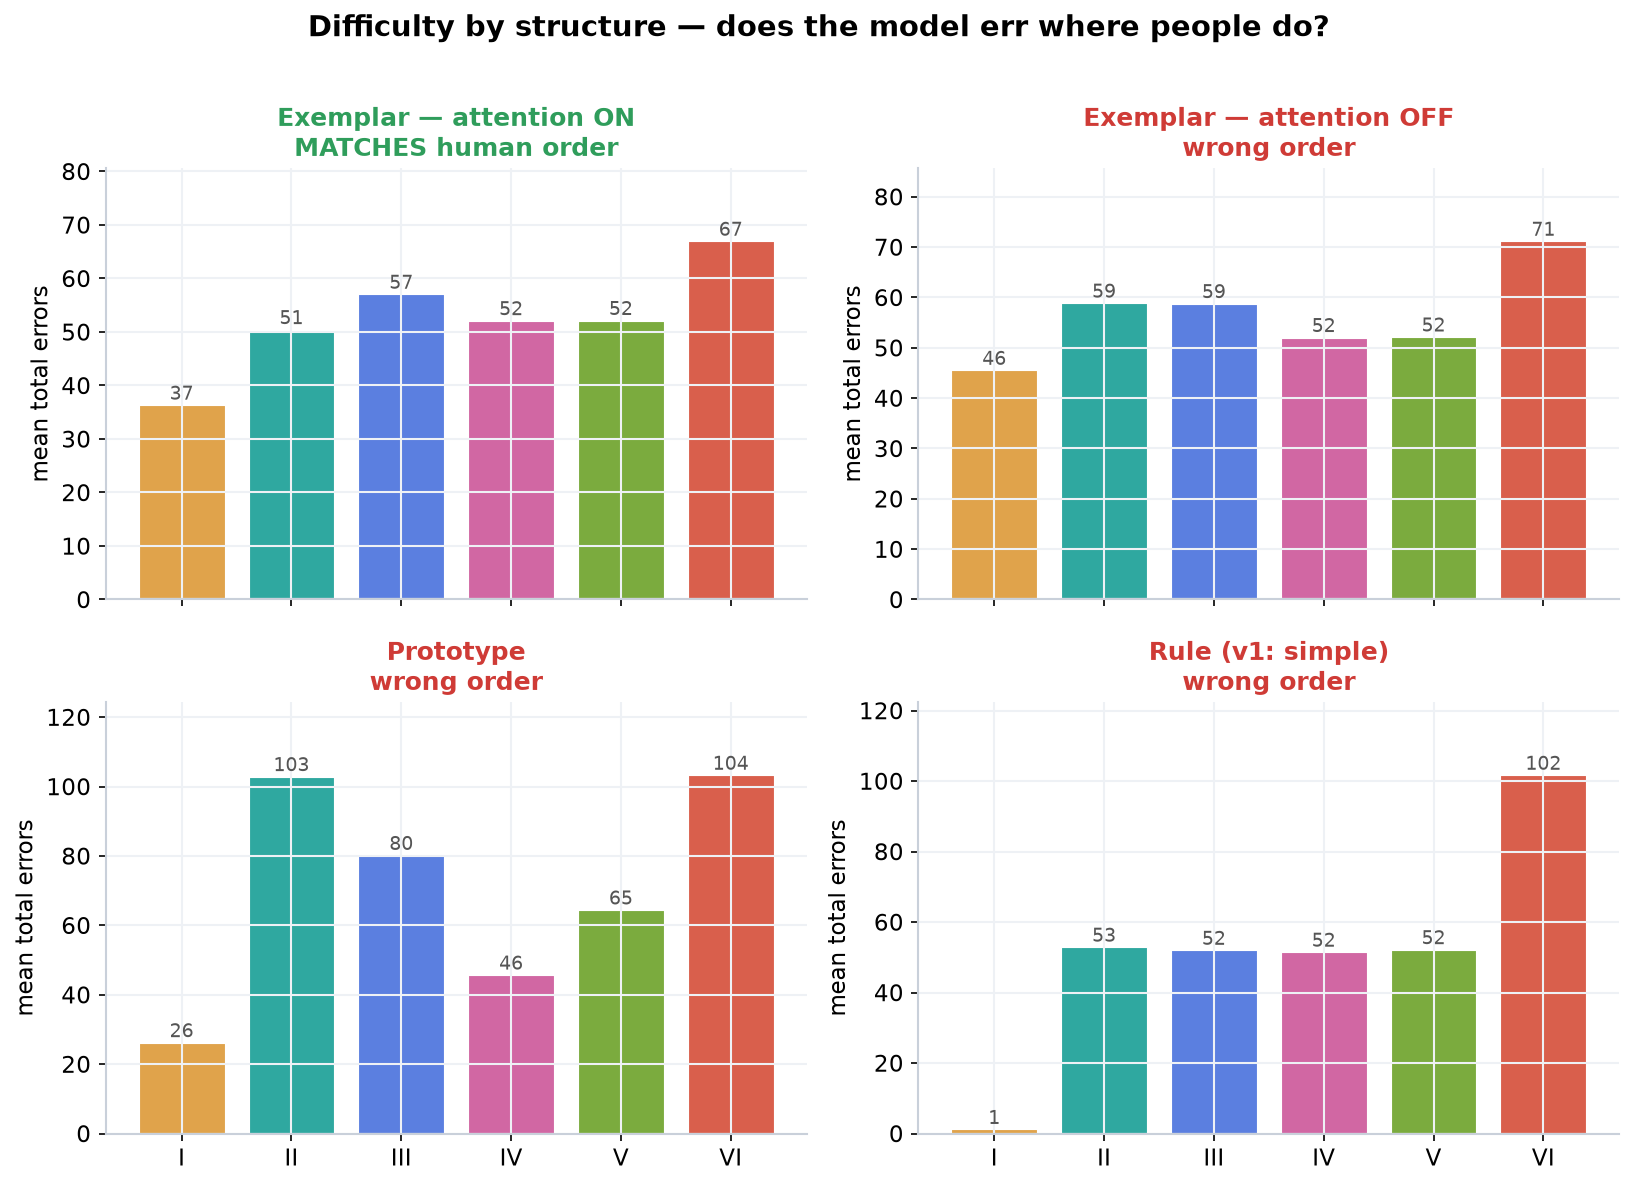
\includegraphics[width=\textwidth]{../figures/fig1_difficulty.png}
\caption{Mean total errors by structure, one panel per model. A panel is marked
as matching the human order when errors satisfy
$\text{I}<\text{II}<\text{band}<\text{VI}$, where band is the mean of Types~III,
IV, and~V. Only the exemplar model with attention matches.}
\label{fig:diff}
\end{figure*}

The Type~II advantage depends on attention specifically. With attention learning
enabled, Type~II is mastered with fewer errors than the III--V band; with
attention frozen and nothing else changed, Type~II rises above that band and the
advantage disappears, while the remainder of the ordering is largely preserved
(Fig.~\ref{fig:attn}). The manipulation therefore localizes the Type~II effect to
the learning of dimensional attention rather than to exemplar storage as such;
storing instances is necessary for the effect but is not by itself sufficient to
produce it.

The prototype model fails where its structure predicts. It learns the
single-feature Type~I readily and the linearly separable Type~IV moderately well,
but it almost never reaches criterion on Types~II and~VI, whose category means
coincide; criterion is reached on roughly eight and seven percent of subjects,
respectively. Its errors are large on the two structures that people find,
respectively, comparatively easy and hardest, so it misorders the middle of the
range and cannot be reconciled with the human pattern.

The rule model presents the opposite profile. It solves Type~I in on the order of
one error per subject, which no other model matches, but it finds Type~II as hard
as the three-dimensional structures and does not reliably reach criterion on
them. Its ordering places Type~II late rather than early, which inverts the human
ordering at precisely the point that most sharply distinguishes the accounts. The
learning curves in Fig.~\ref{fig:curves} show the same result dynamically: the
exemplar-with-attention curves descend on every structure, whereas the prototype
curves for Types~II and~VI do not descend at all.

\begin{figure*}[t]
\centering
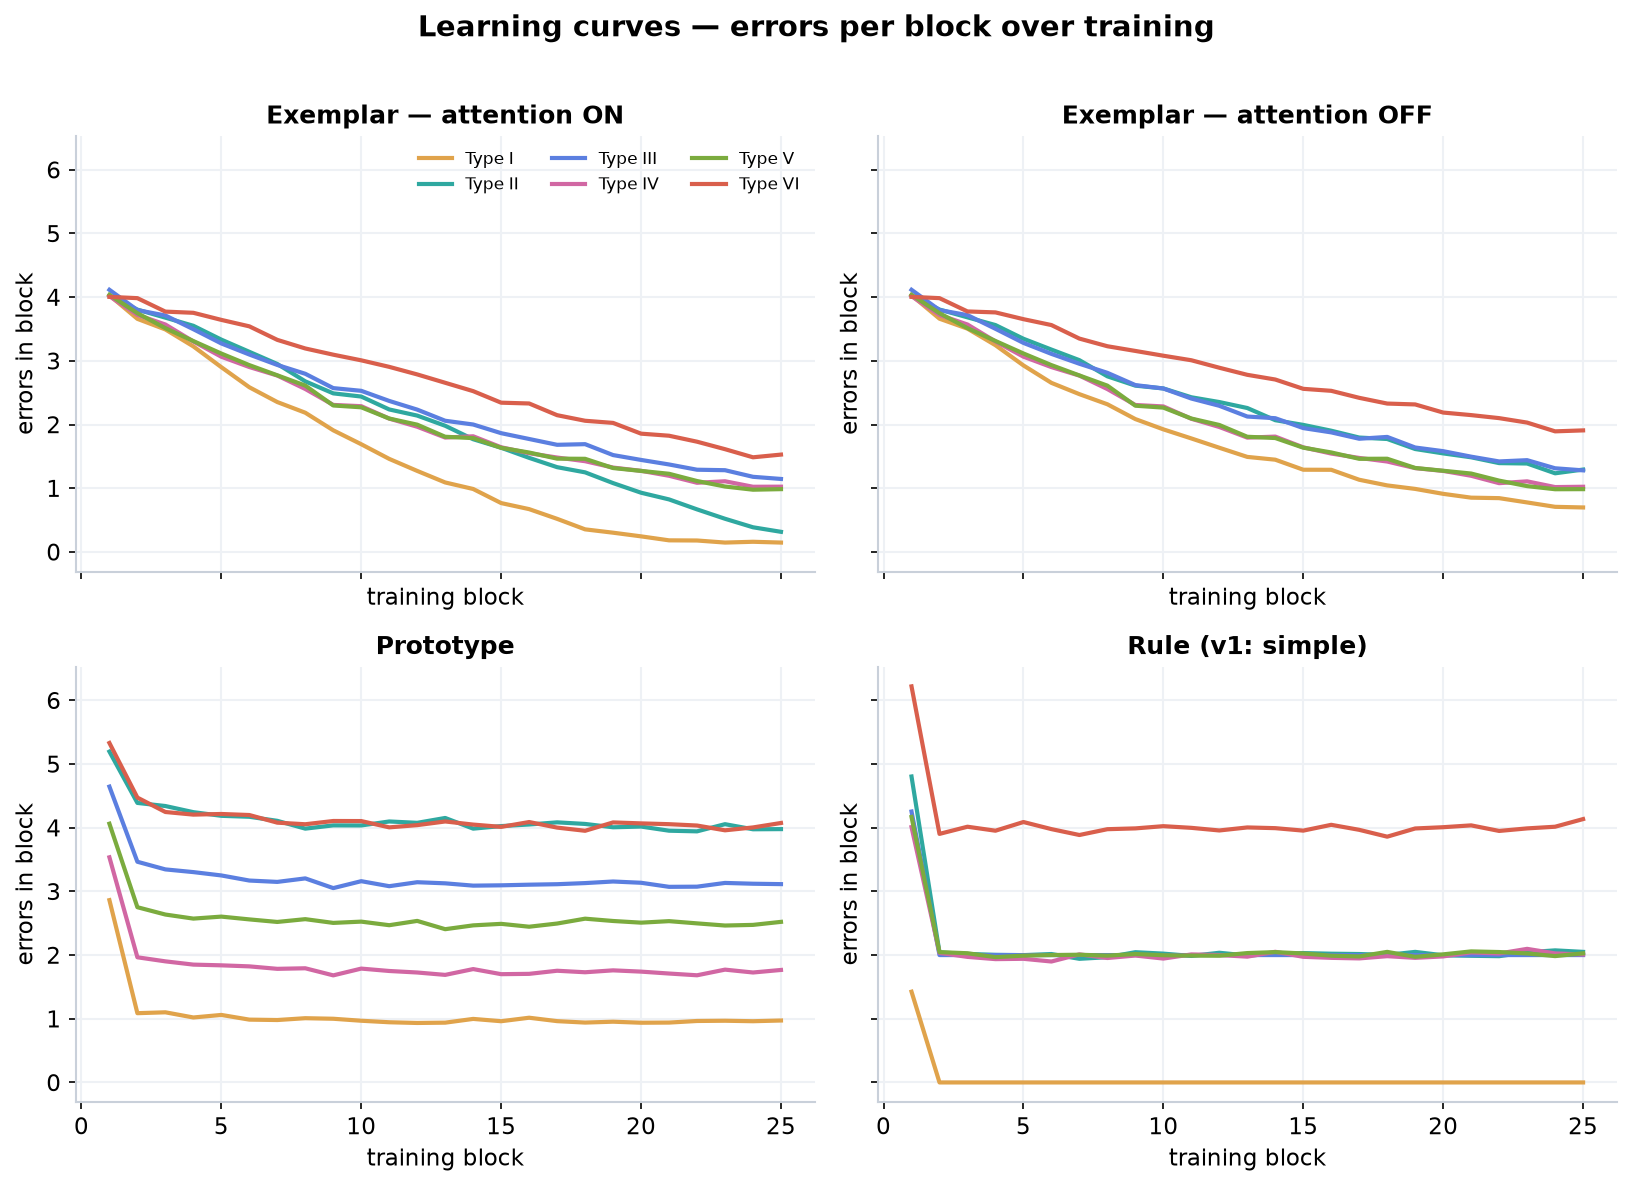
\includegraphics[width=\textwidth]{../figures/fig2_curves.png}
\caption{Learning curves: mean errors per block over 25 training blocks, one
panel per model, one line per structure. Descending curves indicate learning;
the prototype curves for Types~II and~VI remain flat.}
\label{fig:curves}
\end{figure*}

\begin{figure*}[t]
\centering
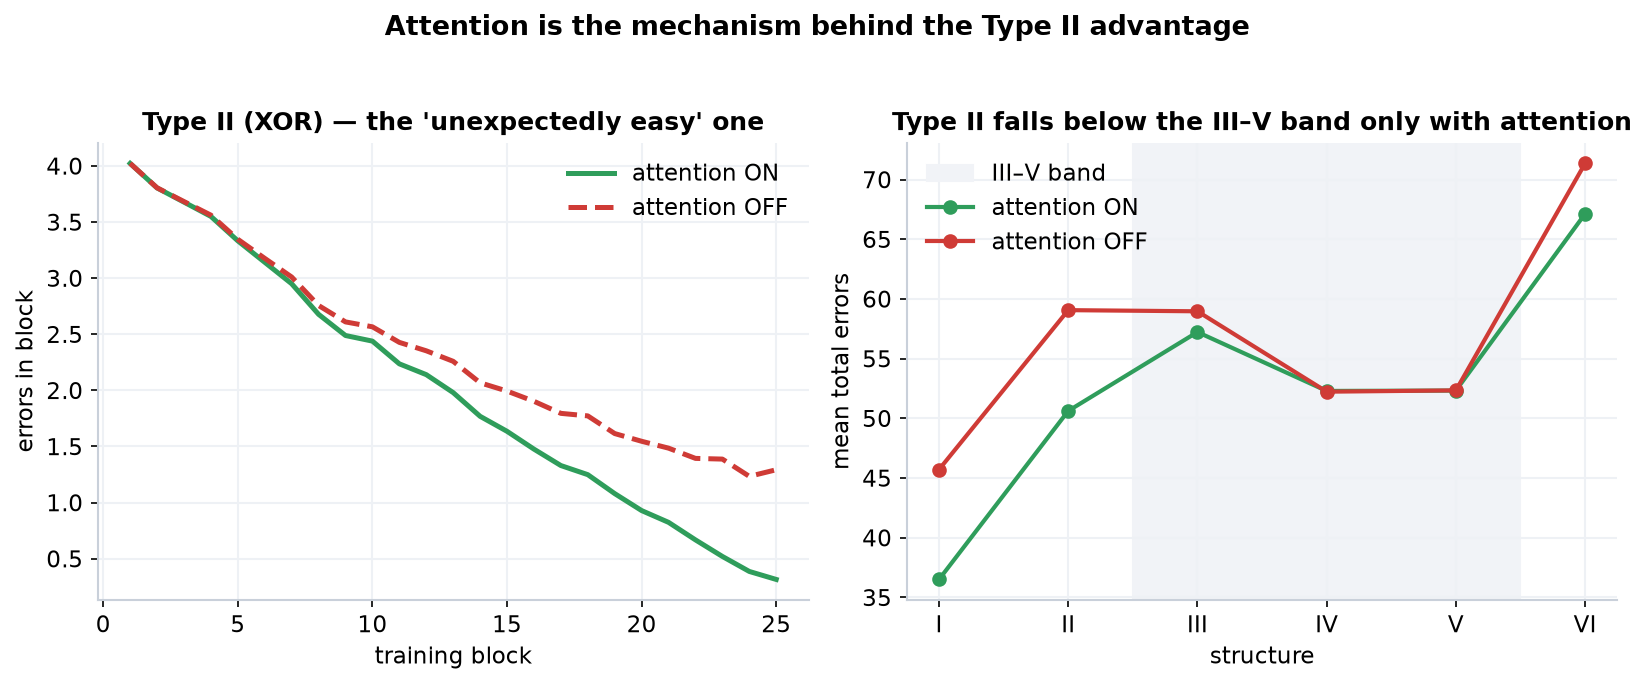
\includegraphics[width=\textwidth]{../figures/fig3_attention.png}
\caption{The attention ablation. Left: the Type~II learning curve with attention
enabled and frozen. Right: total errors by structure for the two conditions, with
the III--V band shaded. With attention frozen, Type~II no longer falls below the
band.}
\label{fig:attn}
\end{figure*}

\section{Discussion}
The results support an exemplar-plus-attention account of human category
learning. The exemplar model reproduces the human ordering only when it can learn
what to attend to, and the ablation shows that this capacity, rather than
instance storage in general, is what makes the Type~II structure easy. The
comparison is informative because the models were built as theories rather than
as tuned classifiers; the prototype model's blindness to Types~II and~VI and the
rule model's inversion of Type~II are consequences of their representational
commitments, not of implementation choices, and they are the behaviors that each
account predicts in advance.

The finding bears on the alignment of machine representations with human ones.
Learned dimensional attention is a mechanism for ignoring irrelevant structure,
and the evidence that machine embeddings match human categories coarsely while
diverging on finer structure \cite{vemuri2025} is consistent with the absence of
such a mechanism rather than with a shortage of data. A representation intended to
generalize as people do, from few examples \cite{lake2015}, would need not only
to store instances but to learn which of their dimensions matter; the Type~II
result is a compact demonstration of why that capacity is necessary.

\section{Limitations}
The rule model is the simplest of the three, and its scope limits the strength of
the rule comparison. A rule-plus-exception account, in which a learner adopts a
simple rule and memorizes the instances that violate it \cite{nosofsky1994rulex},
is a fairer model of human rule use and might narrow the gap on Type~II; the
present rule model therefore establishes a lower bound on what a rule account can
do here rather than the strongest such account.

I reproduce the ordinal difficulty ordering rather than the quantitative human
learning curves. The model parameters were set to standard published values and
were not fit to human data, so the comparison is a test of qualitative ordering,
which is the behavioral signature the benchmark defines, and not a claim of
quantitative fit. Fitting the parameters to published learning curves would be a
stronger test and is left to future work.

The secondary check that most directly separates the prototype and exemplar
accounts, the Medin and Schaffer 5-4 category structure \cite{medin1978}, is
designed but not yet run, because it uses a four-dimensional stimulus set while
the current models are specialized to the three-dimensional SHJ stimuli. The
simulated learners are, finally, not a human replication; the human ordering is
taken from the established literature \cite{shepard1961,nosofsky1994}, and the
contribution is a demonstration of which representational account recovers that
ordering.

\section{Conclusion}
I compared prototype, exemplar, and rule models of concept representation on the
six SHJ category structures and asked which reproduces the human difficulty
ordering. Only the exemplar model with learned selective attention reproduces the
ordering, including the early mastery of Type~II, and an attention-freezing
ablation localizes that advantage to dimensional attention rather than to
exemplar storage in general. The prototype model cannot separate the structures
whose category means coincide, and the simple rule model inverts the human
position of Type~II. Future work extends the rule account to a rule-plus-exception
model, adds the Medin and Schaffer 5-4 check with dimension-general
implementations of the three models, and fits the model parameters to human
learning curves in place of the present ordinal comparison.

\section*{Acknowledgment}
Generative AI (Claude) assisted with phrasing refinement, structural
organization, generation of the figures from my code, identification and
formatting of the scholarly references, LaTeX assembly, and word-count
verification. I selected and verified all references. The research question, the
cognitive science framing, the selection and specification of the models, and the
interpretation of the results are my own.

\bibliographystyle{IEEEtran}
\bibliography{refs}

\newpage
\appendices

\section*{Appendix A: Project Plan Summary}
The plan below follows the course planning template. Total estimated effort is
approximately 70 hours. Milestone deadlines are shown as divider rows. Most
implementation tasks are complete; the Medin and Schaffer 5-4 secondary check and
the presentation deliverables remain.

\begin{table*}[h]
\footnotesize
\centering
\renewcommand{\arraystretch}{1.15}
\begin{tabular}{c c p{0.56\textwidth} c c}
\hline
\textbf{Wk} & \textbf{\#} & \textbf{Task} & \textbf{Hrs} & \textbf{Done} \\
\hline
2 & 1 & Create task list and choose research question & 0.5 & Y \\
2 & 2 & Survey concept-learning literature and confirm tool track / scope & 3.5 & Y \\
3 & 3 & Collect and verify core scholarly references & 1.5 & Y \\
3 & 4 & Write project pitch (all sections) and format in IEEE \LaTeX & 3.5 & Y \\
\hline
\multicolumn{5}{c}{\textit{Project Pitch Due}} \\
\hline
4 & 5 & Set up repository, environment, and project structure & 1.5 & Y \\
4 & 6 & Encode SHJ category structures and stimuli & 3 & Y \\
4 & 7 & Implement the three core models (prototype, GCM/ALCOVE, rule) & 11.5 & Y \\
5 & 8 & Build experiment runner and run models on SHJ structures & 5 & Y \\
5 & 9 & Generate comparison figures and draft optional check-in & 4 & Y \\
\hline
\multicolumn{5}{c}{\textit{Optional Midpoint Check-in Due}} \\
\hline
6 & 10 & Code debugging and architecture refactoring & 7 & Y \\
6 & 11 & Add Medin \& Schaffer 5-4 secondary check & 2.5 & N \\
6 & 12 & Analyze model fit against human difficulty ordering & 3 & Y \\
6 & 13 & Expand reference set to 10+ for final report & 1.5 & Y \\
7 & 14 & Draft full report (abstract through conclusion) & 10 & Y \\
8 & 15 & Revise report, integrate citations, finalize repository & 6 & In prog. \\
8 & 16 & Update project plan and submit final report & 1.5 & In prog. \\
\hline
\multicolumn{5}{c}{\textit{Final Report Due}} \\
\hline
9 & 17 & Build poster and write/rehearse 5-minute script & 4 & N \\
9 & 18 & Record video, assemble submission PDF, verify and submit & 3.5 & N \\
\hline
\multicolumn{3}{r}{\textbf{Total Estimated Hours}} & \textbf{73} & \\
\hline
\end{tabular}
\end{table*}

\section*{Appendix B: Code Repository}
The complete implementation---the stimulus and structure encoding, the three
models, the experiment runner, the reproducible analysis notebook, and the test
suite that verifies the six category structures by enumeration---is available at
the private course repository:
\begin{center}
\url{https://github.com/RabeaWahab/gt-cs6795-concept-learning}
\end{center}
The repository includes a \texttt{README.md} with setup and execution
instructions; the reported figures and numbers are regenerated by running the
notebook \texttt{notebooks/model\_comparison.ipynb} from a fixed random seed.

\end{document}
